\documentclass[oribibl,runningheads,a4paper]{llncs}

\usepackage{amssymb}
\setcounter{tocdepth}{3}
\usepackage{graphicx}
\usepackage[numbers, square, sectionbib]{natbib}
\usepackage{color}

\usepackage{url}
\urldef{\mailsa}\path|blaz.skrlj@ijs.si, jan.kralj@ijs.si, anze.vavpetic@jis.si, nada.lavrac@ijs.si|
\usepackage{amsmath}
\DeclareMathOperator*{\argmax}{arg\,max}

\newcommand{\keywords}[1]{\par\addvspace\baselineskip
\noindent\keywordname\enspace\ignorespaces#1}

\begin{document}

\mainmatter  % start of an individual contribution

% first the title is needed
\title{Community-based semantic subgroup discovery}

% a short form should be given in case it is too long for the running head
\titlerunning{Lecture Notes in Computer Science: Authors' Instructions}

\author{Bla\v{z} \v{S}krlj\inst{2}%%
\and An\v{z}e Vavpeti\v{c}\inst{1} \and Jan Kralj\inst{1,2} \and Nada Lavra\v{c}\inst{2,3}}
%
\authorrunning{\v{S}krlj, Vavpeti\v{c} et al.}
% (feature abused for this document to repeat the title also on left hand pages)

% the affiliations are given next; don't give your e-mail address
% unless you accept that it will be published
\institute{Jo\v{z}ef Stefan Institute, Jamova 39, 1000 Ljubljana, Slovenia\\ 
\and Jo\v{z}ef Stefan Int. Postgraduate School, Jamova 39, 1000 Ljubljana, Slovenia
\and University of Nova Gorica, Vipavska 13, 5000 Nova Gorica, Slovenia\\
\email{\mailsa}}


\toctitle{Lecture Notes in Computer Science}
\tocauthor{Community-based semantic rule induction}
\maketitle


\begin{abstract}
Semantic subgroup discovery leverages the background knowledge in form of ontologies to augment the subgroup discovery process. The input for such methodology normally consists of manually created classes of instances, provided by domain experts. We present an algorithm we termed CBSSD (community-based semantic subgroup discovery), which identifies possible classes of instances based on structural properties of complex networks related to the studied phenomenon. Furthermore, obtained classes are used in the process of semantic subgroup discovery. The application of the developed procedure is demonstrated on two motivating examples from the field of molecular biology. Automatically obtained rulesets cover the majority of knowledge, previously retrieved via manual literature inspection by domain experts.
\keywords{Semantic data mining, bioinformatics, knowledge discovery}
\end{abstract}

\section{Introduction}

Modern machine learning approaches are capable of using ever-increasing amounts of information to explain complex phenomena from the fields of biology, sociology, mechanics and electrical engineering. As there can be many distinct types of data associated with a single phenomenon, novel approaches strive towards integration of different, heterogeneous data sources into unified models. Aim of this work is to propose a methodology, where iteratively constructed complex networks are used to identify relevant subgroups, which are used as input for the process of semantic subgroup discovery. We demonstrate that new knowledge can be obtained using existing, freely accessible heterogeneous data in form of complex networks and ontologies. \\
\indent In further sections we introduce the notions of background knowledge in machine learning, ontologies, complex networks, and semantic subgroup discovery. We continue with an in-depth explanation of the proposed approach. Finally, we demonstrate the use of proposed methodology on two datasets from the life science domain, where complementarity with existing enrichment analysis tools is demonstrated.

\section{Using background knowledge in machine learning}

Modern machine learning (ML) methodology is becoming more complex, as the size and the speed of incoming data increases exponentially. In such settings, prior knowledge can play a big role in the development and deployment of learning algorithms in a real world setting. Background knowledge can come in many forms, which introduces additional complexity to the modeling process, yet can have a large impact on the model's performance. For example, Bayesian methodology is can be leveraged to incorporate knowledge about prior states of a system - prior distributions of random variables being modeled. In the Bayesian setting, the prior knowledge is incorporated via conditional probabilities and the Bayes' rule. The posterior probability of event A, given event B can be described as $P(A|B) = \frac{P(B|A)P(A)}{P(B)}$, where the P(B) is a normalizing constant, normally left out, so the equation becomes $ P(A|B) \approx  P(B|A) P(A) $. Methodology from different fields already uses similar approaches for solving ML problems. For instance, \citeauthor{Madahian2015} \cite{Madahian2015} report a method, where the general linear model was developed to aid gene expression profiling. They achieved better predictive accuracy by using prior knowledge based on the index rank of the term "cancer" in underlying background knowledge. Bayesian methodology is also in widespread use in the field of phylogenetics, where Bayesian inference is used for reconstruction of evolutionary trees \cite{drummond2007beast,huelsenbeck2001mrbayes,zou2005new}. Another machine learning discipline, which relies heavily on the use of background knowledge is inductive logic programming (ILP) \cite{lavrac1994inductive}. In ILP, background knowledge is used along with examples to derive logical programs, which cover all positive examples. 

\subsection{Ontologies}
Background knowledge can also be introduced to the model using curated domain knowledge in the form of ontologies. An ontology can be represented as a data structure consisting of semantic triplets $T(S,P,O)$, which represent the subject, its predicate and the targeted object. Resource description format hypergraph (RDF) is a data model commonly used to operate at the intersection of data and the ontologies. There are many existing approaches, which use background knowledge in the form of an ontology to obtain either more accurate or more general results \cite{Dou2015}. First, knowledge in the form of ontologies can represent constraints, specific to a domain. It has been empirically and theoretically demonstrated, that using background knowledge as a constraint can improve general classification performance \cite{balcan2013exploiting}. The RDF framework provides the necessary formalism to leverage the graph-theoretic methods for ontology exploration. Random walk approach and large scale sampling are some of the techniques used to discover indirectly associated biological terms \cite{liu2013mining}. Semantic clustering is an emerging field, where semantic similarity measures are used to determine the clusters using the background knowledge \cite{hotho2002ontology}, in a manner similar to, for example, $k$-means family of clustering algorithms. Semantic clustering is frequently used in the area of document clustering \cite{hotho2002ontology}. Performance gains in precision, consistency of results and recall were reported for many text mining algorithms \cite{jing2010knowledge}. Large databases in the form of RDF triplets exist for many domains. For example, the Bio2RDF project \cite{belleau2008bio2rdf} aims at integrating all major biological databases and joining them under a unified framework, which can be queried using SPARQL - a specialized query language. In this sense, Bio2RDF serves as an integrated database of biological information, yet there remain opportunities to exploit the aggregated knowledge.

\subsection{Complex networks}

Many natural phenomena can be described using graphs. Complex networks are graphs with distinct, real world topological properties \cite{cohen2010complex}. They can be used to model physical, biological, chemical and mechanical systems \cite{palla2005uncovering}. Real world networks can be characterized with distinct statistical properties regarding their node degree distribution, component distribution or connectivity \cite{strogatz2001exploring}. Complex biological and social networks are also known to include many communities -- smaller, distinct units of a network \cite{duch2005community}.

\subsection{Semantic subgroup discovery (SSD)}

Subgroup discovery is a machine learning discipline which can be described as a combination of supervised and unsupervised learning. Subgroup discovery in general can be considered as a part of rule learning paradigm. Algorithms expect a labeled training set, where class labels are used to denote the groups for which descriptive rules are to be learned. Subgroup discovery was extended to semantic subgroup discovery (SSD) \cite{vavpetivc2013semantic,trajkovski2006relational,langohr2012contrasting}, where the semantic learner, apart from experimental data, also leverages background knowledge in the form of ontologies in order to guide the rule learning process. The Hedwig algorithm \cite{adhikari2016explaining, vavpetivc2013semantic} for example, accepts the input in form of ontologies and instances, grouped into target classes. Individual instances are mapped into the ontology domain, where Hedwig is capable of using arbitrary ontology to identify latent relations between individual instances.


\section{Methodology}

In this following section we describe a three step approach for semantic subgroup discovery from complex networks we termed CBSSD (community-based semantic subgroup discovery). Proposed approach operates on a list of terms connected with the studied phenomenon. The steps include: network construction, community detection and semantic subgroup discovery. The proposed methodology is depicted in Figure~\ref{fig:example}. 

\begin{figure}[!h]
\centering
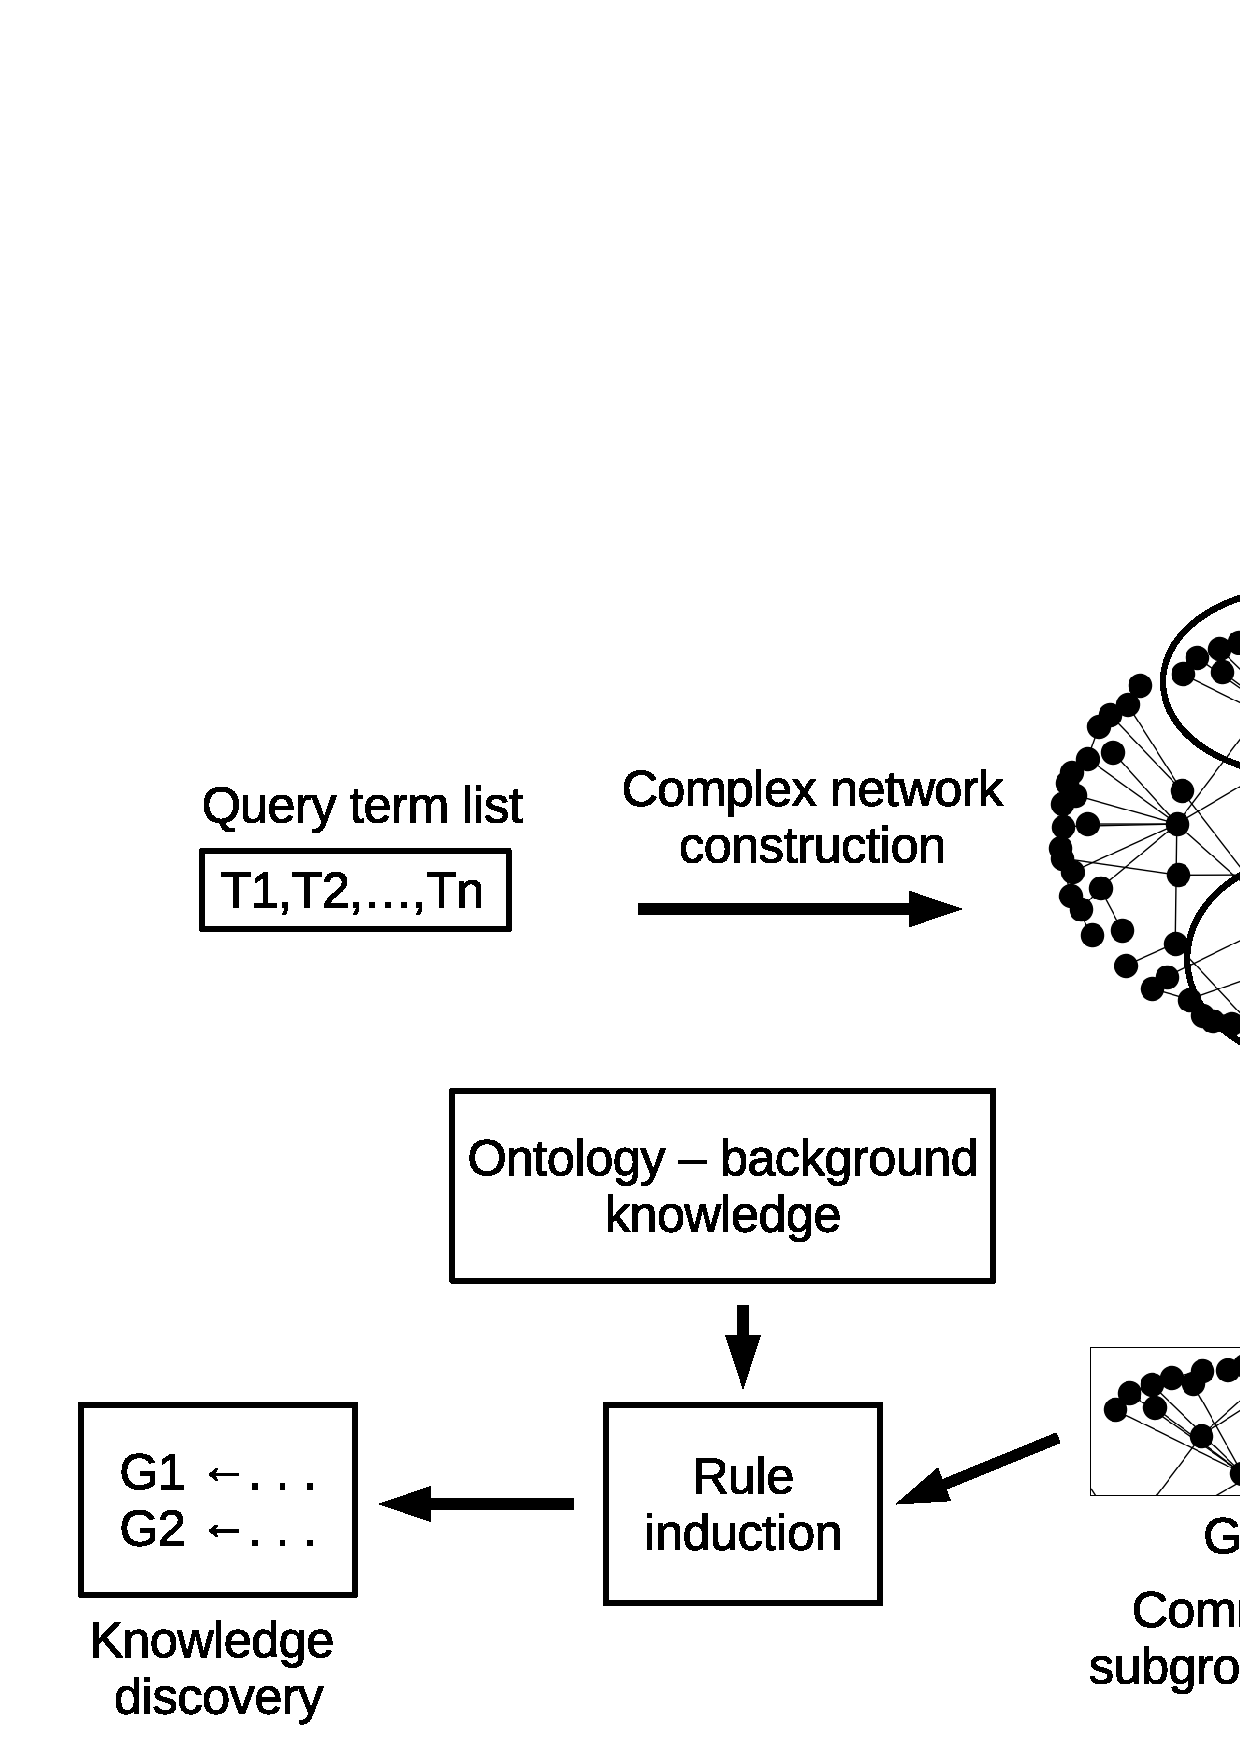
\includegraphics[scale=0.35]{workflow2}
\caption{Schematic representation of the proposed CBSSD procedure. A complex graph's communities are used to identify possible subgroups in the input term list. The subgroups are further explained using semantic subgroup discovery with background knowledge.}
\label{fig:example}
\end{figure}

\subsubsection{Constructing the network of associations}
A list of relevant biological terms is used to construct a term network. The network is constructed using the BioMine methodology \cite{eronen2012biomine}. Individual terms are used as seeds for crawling the BioMine knowledge graph, which already includes term associations across main biological databases, such as UniProt \cite{uniprot2014uniprot}, Kegg \cite{kanehisa2000kegg}, and GenBank \cite{benson2012genbank}. Final knowledge graph is constructed incrementally, by querying one term at a time. The final result is a set of graphs $\{G_1,\dots, G_n\}$, where $n$ is the number of total query terms and, for each $i$, $G_i=(V_i, E_i)$. In order to obtain the final graph $G_f$, node and edge information from $\{G_{1},..,G_{n}\}$ is joined into a single graph. Throughout the network construction process, nodes and edges can not be duplicated - once the node is present in the final graph, only new edges can be added. Final set of nodes $V_{f}$ thus equals $\bigcup_{i=1}^{n}V_{i}$ and final set of edges $E_{f}$ similarly equals to $\bigcup_{i=1}^{n} E_{i}$. 


\subsubsection{Subgroup identification using community detection}

Once the network is constructed, network community detection is used to identify interesting subsets of the network, which are directly mapped to groups within the input query list. We use the Louvain algorithm \cite{blondel2011louvain}, which is based on the network modularity measure \cite{newman2006modularity},  defined for split into two modules ($m_{i}$ and $m_{j}$) as:

\begin{equation}
\xi = \frac{1}{2m}\sum_{i=1}^n\sum_{j=1}^n \bigg[A_{i,j} - \frac{d_{i}d_{j}}{2m} \bigg]\frac{m_{i}m_{j}+1}{2}
\end{equation}


\noindent where the $\xi$ represents the modularity, $m$ the number of all edges, $A$ the adjacency matrix (i.e., $A_{ij}$ is equal to $1$ if the $i$-th and $j$-th node are connected and $0$ if they are not), and $d_{i}$ is the degree of node $u_i$. The term $m_i$  represents a membership function which returns $1$ if a specific node is present in the observed module and $-1$ otherwise. The final community partition includes all nodes. The Louvain algorithm is one of the most scalable community detection methods due to its $O(nlog(n))$ time complexity. For this step, the constructed knowledge graph was interpreted as an undirected graph, which is a feasible assumption as long we are interested only in biological associations. The community detection procedure returns sets of nodes $C_{1\dots n}$, representing individual communities. Each node in the network belongs to exactly one community (i.e., the communities are non-overlapping). We are interested in finding subgroup descriptions of these communities. In order to do this, each community $C_i$ becomes a class label $T_i$. The terms from the input list are partitioned to individual classes according to the community they belong in. This way, input terms are grouped into distinct classes, yet no additional terms are added as they could introduce unnecessary noise in the semantic subgroup discovery step.

\subsubsection{Preparation of the background knowledge}

Semantic rule learning requires the data to be encoded in the form of semantic triplets $T(S,P,O)$, where $S$ is the subject, $P$ the predicate and $O$ the object. The experimental data from the previous step was converted to triplets in accordance with Hedwig, the algorithm used in the rule discovery process \cite{vavpetivc2013semantic}. Hedwig is capable of leveraging the background knowledge in form of ontologies to guide the rule construction process. As the CBSSD methodology is primarily developed for the field of bioinformatics, our main source of background knowledge in this study is the Gene ontology \cite{ashburner2000gene} database, one of the largest semantic resources for biology. It includes tens of thousands of terms, which together form a directed acyclic graph, directly usable by SDM tools. For Hedwig to generalize, two conditions must be met. First, individual term names from the community detection step need to have the corresponding GO term associations, and second, the whole gene ontology must be provided as a source of background knowledge. This step requires discovered communities to be encoded in form of semantic triplets. Such encoding is achieved by treating the observed community as an individual target class, where all of its terms are considered as instances of that class. The key aspect of the rule generation procedure is the definition of the predicate, which will be used for finding suitable rule conjunctions. The objective function is thus  Learn a rule set $\Delta$  for individual classes $\zeta_{1,..,n}$ using background knowledge ($\Xi$) in form of ontologies and class instance embeddings $\gamma$, such that the likelihood of individual class representations $\zeta_{x};x \in \{1,..,n\}$ is maximized.

\begin{equation}
\Delta_{\zeta_{1},..,\zeta_{n}} = \argmax_{i \in \{1,..,n\}}\Big[P(\Delta_{\zeta_{i}}|\Xi,\gamma) \Big]
\end{equation}

By convention, we use the \emph{subClassOf} predicate when constructing the knowledgebase for Hedwig algorithm. Individual rules' p-values are determined by Fisher's exact test, a non-parametric, contingency table-based procedure, where a difference in coverage between two rules is leveraged to select the better one.

\section{Applications of the developed procedure}

In this section, we demonstrate the use of the proposed methodology on two real datasets from the life science domain. First, we consider properties of amino-acid variants within protein binding sites, followed by proteins identified in the context of epigenetics. %evo super, ta stavek mi je manjkal.


\subsection{Properties of proteins with single amino-acid variants present in the binding sites}

Sequence variants are nucleotide or amino acid substitutions, that can lead to unstable protein interaction complexes and thus influence the organism's phenotype (e.g., induce a disease state). There are two main types of variants, polymorphisms or germ-line variants, which are heritable, and somatic mutations, which appear in somatic tissues without previous genetic encoding. Although it was demonstrated that variants within biological interactions can be associated with disease occurrence \cite{skrlj2017,skrlj2016computational,schroder2005single,kamburov2015comprehensive}, currently there are no studies which would study this phenomenon to discover new subgroups of proteins associated with variants within interaction sites at a more general level. We use  results from a previous enrichment analysis study \cite{skrlj2017} for comparison with the proposed methodology. Results are compared based on terms appearing in both approaches, i.e. terms found as a result of enrichment analysis as well as as a result of semantic subgroup discovery. As the two approaches compared are fundamentally different, intersection of both results is expected to be relatively small (only very significant terms).

\subsubsection{Preparing the input for semantic subgroup discovery}

More than 300 UniProt terms, for which variants were found within protein binding sites were used as the input query list (found in supplementary material of \cite{skrlj2017}). A BioMine network with more than 1,650 nodes and 2,300 edges was constructed. The resulting network is depicted in Figure~\ref{fig:example2} using two possible visualizations. 

\begin{figure}[!t]
\centering
\includegraphics[scale=0.52]{combined_biomine_grayscale}
\caption{Final size of the BioMine network, associated with polymorphisms located within protein interaction sites. Image A) contains the multiplex view of the final network and B) the network modules in using standard, force-directed layout.}
\label{fig:example2}
\end{figure}


Triplet construction consists of first mapping the nodes from the knowledge graph to associated ontology terms, and second, the construction of the background knowledge. For this demonstration, gene ontology \cite{ashburner2000gene} was used in both steps. 
Semantic subgroup discovery was conducted for more than $20$ communities, and as the main result, more than $100$ rules of various lengths were obtained. The most significant and the longest rules were manually inspected to identify possible overlap with previous pathway enrichment studies done on the same input dataset. Different beam sizes were experimented with in the procedure (from $10$ to $50$). 

\begin{table}[!t]
\centering
\caption{Gene ontology terms, found  both in enrichment and semantic rule learning process. Terms marked with "*" are statistically significant ($p < 0.1$) and therefore the most relevant for semantic subgroup discovery.}

\label{table:results}
\begin{tabular}{|c c|}
\hline
Gene ontology term & Meaning                              \\ \hline 
GO:0000077         & DNA damage checkpoint*                \\ 
GO:0000086         & Mitotic cell cycle*                   \\ 
GO:0003677         & DNA binding*                          \\ 
GO:0004871         & Signal transducer activity*           \\ 
GO:0005730         & Nucleolus*                            \\ 
GO:0005814         & Centriole                            \\ 
GO:0016020         & membrane                             \\ 
GO:0016605         & PML body                             \\ 
GO:0030018         & Z-disc                               \\ 
GO:0035264         & Multicellular organism growth        \\ 
GO:0045892         & Negative regulation of transcription (DNA) \\ 
GO:0000122         & Negative regulation of transcription (RNA) \\ 
GO:0000785         & Chromatin                            \\ \hline
\end{tabular}
\end{table}


\subsubsection{Results}

The obtained rule-sets for identified communities were further investigated. We directly compared the ontology terms present in the rules with terms, identified as significant in our previous study \cite{skrlj2017}. For this na\"ive comparison, conjuncts were considered as individual entries, as we were only interested in term presence (not coverage). There were $13$ gene ontology terms present in both approaches (Table~\ref{table:results}).


Although only 13 terms were found with both procedures, the identified terms were among the most significant ones detected in the enrichment analysis setting. This indicates, that both procedures identified a strong signal related to DNA and cell cycle related processes. As semantic subgroup disovery was conducted for separate communities, the results were expected to be more detailed and comprehensive. This was indeed the case: there were many rules consisting of two conjuncts, such rules can be more informative than the ones identified by ontology enrichment analysis. As iron binding proteins were present in the protein list (this was known from the previous study \cite{skrlj2017}), a rule $R=$ \emph{GO:0034618} $\wedge$  \emph{GO:0006874} appeared as one of the most significant rules ($p<0.1$). Ontology terms in this rule represent arginine binding and cellular calcium homeostasis - both processes indeed involve terms from the part of the input term list; a part not directly detected with enrichment analysis. The key UniProt term found for this rule was P41180 (CASR), which represents the extracellular calcium-sensing receptor \cite{garrett1995molecular}. As CASR is indeed critical for calcium homeostasis discovery (GO:0006874), it serves as an indicator of the validity of our CBSSD approach. The second term (GO:0034618), representing arginine binding is not so directly associated with the CASR protein. To further investigate the context, within which GO:0034618 occurs, we queried the gene ontology database directly for similar proteins, already associated with this term. The majority of proteins, annotated with this term, correspond to acetylglutamate kinase, an enzyme that participates in the metabolism of amino acids (e.g., urea cycle). A possible interpretation of this association is that as the CASR protein induces hormonal response, which could effectively lead to increased amino-acid metabolism, providing the molecular components necessary for establishment of homeostasis. This association serves as a possible candidate for further experimental testing and demonstrates the hypothesis generation capabilities of proposed approach. Schematic representation of discussed results is presented in Figure~\ref{fig:example3}.\\

\begin{figure}[!h]
\centering
\includegraphics[scale=0.9]{result_nicer}
\caption{Comparison of ontology terms discovered by CBSSD approach and conventional enrichment analysis (whole term list). Only significant rules were used in visualization ($p<0.1$), hence only 5 common terms are depicted in the term matrix (down-right part of the image).}
\label{fig:example3}
\end{figure}

Another interesting rule emerged from the first community identified. The rule \emph{GO:0030903 $\wedge$  GO:0000006} was found for UniProt entries Q96SN8  (CDK5 regulatory subunit-associated protein 2), O94986 (Centrosomal protein), Q9HC77 (Centromere protein J) and O43303 (Centriolar coiled-coil protein). As it can be observed, all the identified proteins are connected with nucleus-related processes. Term \emph{GO:0030903} corresponds to notochord development, which is a stage in cell division - a term directly associated with identified proteins. The second term, \emph{GO:0000006}, corresponds to high-affinity zinc uptake transmembrane transporter activity, a process related to enzyme system responsible for cell division and proliferation. Although this rule does not imply any new hypothesis, it demonstrates the generalization capability of the proposed approach. To further emphasize the difference between conventional enrichment analysis and our approach, we visualize the term matrix for both approaches (Figure~\ref{fig:example3}) along with schematic workflows. From the visualization it can be observed that only a minority of terms are covered by both approaches, whereas many terms remain specific for either semantic rule discovery based on community detection or enrichment analysis. This discrepancy appears due to the fact that community detection splits the input term list into smaller lists, which can be described by completely different terms than the list as a whole. As the proposed methodology splits the input list, it is not sensible to compare it with conventional approaches, which operate on whole lists. The GO term comparison in Figure~\ref{fig:example3} serves only as a proof of fundamental difference between the two approaches. Nevertheless, we deem our approach to be an useful complementary methodology to well established enrichment analysis.


\subsection{Grouping of epigenetic factors}
Epigenetics is a subfield of genomics, where processess such as methylation are studied in the context of the influence of environment on the phenotype. Epigenetic factors are actively researched, and are constantly updated in databases such as emDB \cite{nanda2016dbem}, where many information such as gene expression, tissue information and variant information are publicly accessible. We tested the developed approach on the list of all currently known epigenetic factors \cite{nanda2016dbem}. The epigenetics dataset was chosen for two main reasons: 1.) to demonstrate the CBSSD's performance on a dataset, to our knowledge not yet used in semantic subgroup discovery and 2.) this dataset serves to further test the developed mehodology in the context of different biological process. The 153 distinct UniProt terms were used as input for the BioMine knowledge graph construction. Final graph consisted of ~4,500 nodes and ~5,500 edges, respectively. The obtained knowledge graph is significantly larger than the one used in the previous case study (properties of SNVs in binding sites) and thus demonstrates the capabilities of the developed approach on larger graphs. More than 50 communities were identified and further inspected. For the community, which includes UniProt term Q8WTS6 (Histone-lysine N-methyltransferase), many interesting rules emerged. For example, the most significant rule ($p=0.09$): \emph{GO:1990785 $\wedge$ GO:0000975 $\wedge$ GO:0000082} indicates, that the protein is indeed highly associated with epigenetic processes. Term \emph{GO:1990785} describes water-immersion restraint stress, term \emph{GO:0000975} regulatory region DNA binding and term \emph{GO:0000082} transition of mitotic cell cycle. All three terms exactly describe the Q8WTS6 entry, as it effects the DNA's topological properties (coil formation) and is responsible for transcriptional activation of genes, which code for collagenases, enzymes crucial to mitotic cell cycle (wall formation). This example demonstrates that at least the most significant rules found directly describe the underlying biological process, yet other rules diverge from the enrichment analysis - similarly to the sequence variant example.


\section{Conclusions and further work}
Semantic data mining is an emerging field, where background knowledge in the form of ontologies can be used to generalize the rules emerging from the learning process. In this study, we demonstrate how such an approach can be used to induce rules describing the communities, detected on an automatically constructed knowledge graph. Our implementation was tested on two datasets from the life science domain, where validity of the most significant rules was manually inspected in terms of biological context. This approach works for up to 2,000 terms in reasonable time (e.g. a day), but for more than e.g., 10,000 terms, whole graphs should be used from the beginning if possible. As the number of rules produced can be large, adequate visualization techniques for elegant result inspection are still to be developed. \\
Our approach differs significantly from conventional enrichment analysis, as interesting groups of terms are identified based on the underlying network structure, rather than manual, expert-guided selection. The proposed CBSSD approach is still to be extensively tested. We currently see it as a complementary methodology to enrichment analysis, as it is capable of describing latent patterns beyond the ones expected by a domain expert. \\
Although we demonstrated, that CBSSD approach can provide useful insights in the field of molecular biology, our further work will be aimed at generalization this methodology to arbitrary problems from other fields, such as natural language processing. As ontologies are not necessarily well developed, we will further explore the options of automated ontology generation from complex networks, a data type available in majority of scientific fields.\\
As our approach detects communities on a simplified networks, we believe further improvements can be achieved via the use of some of the recent multiplex community detection approaches.

%%% Further work...
\subsubsection*{Acknowledgments.} 

This research work is supported by Slovenian Research agency (ARRS).

\bibliography{references} 
\bibliographystyle{apalike}


\end{document}
